\documentclass{article}

\usepackage[spanish]{babel}
\usepackage{fontenc}
\usepackage[utf8]{inputenc}
\usepackage{hyperref}
\usepackage{graphicx}
\usepackage{amsmath}
\usepackage{amsfonts}
\usepackage{amssymb}
\usepackage{amsthm}
%\usepackage[left=30pt,right=40pt,top=40pt,bottom=60pt]{geometry}

\author{NyKi}
\date{Enero 2025-}

% Entornos
\theoremstyle{definition}
\newtheorem{theorem}{Teorema}
\newtheorem{prop}{Proposición}
\newtheorem{cor}{Corolario}
\newtheorem{lemma}{Lema}
\newtheorem{axiom}{Axioma}
\newtheorem{define}{Definición}
\newtheorem{note}{Nota}
\newtheorem{ejem}{Ejemplo}

\DeclareMathOperator{\trace}{tr}

% Conjuntos
\newcommand{\reales}{\mathbb{R}}
\newcommand{\naturales}{\mathbb{N}}
\newcommand{\racionales}{\mathbb{Q}}
\newcommand{\cinfinito}{\mathcal{C}^{\infty}}
\newcommand{\claseck}[1]{\mathcal{C}^{#1}}


\begin{document}

Estas notas proporcionan un estudio elemental de las curvas y las superficies, como se presenta en un primer curso de geometría diferencial.

\section{Preliminares de análisis y geometría}
Por comodidad, asumiremos que $\naturales$ (el conjunto de los números naturales) empiezan en el $1$ (es decir, no contienen al $0$).

\begin{define}
	Una aplicación $f:U\subseteq\reales^n \rightarrow \reales^m$ con $n,m$ enteros mayores a 0 y $U$ abierto no vacío se denomina \textbf{de clase $\claseck{k}$} si admite parciales hasta el orden $k \in \naturales$ y estas son continuas.
\end{define}
\begin{define}
	Una aplicación $f:U\subseteq\reales^n \rightarrow \reales^m$ con $n,m$ enteros mayores a 0 y $U$ abierto no vacío se denomina \textbf{de clase $\cinfinito$} si admite parciales de todos los órdenes y estas son continuas.
\end{define}
Es un resultado de un curso de análisis que una aplicación $\cinfinito$ definida sobre un dominio abierto es diferenciable. Otro nombre para las funciones $\cinfinito$ es suave.
\begin{define}
	Una aplicación $f:I \rightarrow J$ con $I,J$ intervalos abiertos de números reales se dice $difeomorfismo$ si es biyectiva, derivable y su inversa también es derivable.
\end{define}
De la definición se puede ver que un difeomorfismo es también un homeomorfismo.

\section{Curvas parametrizadas}


\begin{define}
	Decimos que una aplicación $\alpha: I \rightarrow \reales^2$ (con $I$ un intervalo abierto de $\reales$) de clase $\cinfinito$ es una \textbf{curva parametrizada diferenciable} (o paramétrica). El conjunto $\alpha(I)$ se denomina \textbf{traza} de la curva y lo denotamos mediante $\trace(\alpha)$.
\end{define}
Hemos de notar que la condición de ser $\cinfinito$ es muy fuerte. Podríamos perfectamente requerir solo que fueran $\claseck{k}$ para algún $k \in \naturales$, y de hecho algunos ejemplos trataremos estas curvas, pero requerir diferenciabilidad infinita hace el trabajo teórico más fácil. En esta definición nos hemos restringido a intervalos abiertos de la recta real. Es posible considerar intervalos cerrados, pero nos tenemos que asegurar que la función en los extremos se pueda ``extender'':
\begin{define}
	Decimos que una aplicación $\alpha: I \rightarrow \reales^2$ (con $I$ un intervalo cerrado de $\reales$) de clase $\cinfinito$ es una \textbf{curva parametrizada diferenciable} si existe una curva paramétrica diferenciable $\beta: I^* \rightarrow \reales^2$ definida sobre un intervalo abierto $I^*$ que contiene a $I$ tal que $\beta  \big|_I = \alpha$ y $\beta^{(k)}  \big|_I = \alpha^{(k)}$ para todo $k \in \naturales$.
\end{define}
Aunque esta definición presenta algún que otro problema, como veremos al hablar de curvas cerradas. Cuando hablemos de curvas definidas sobre un intervalo, simplemente asumiremos que es abierto.
Veamos algunos ejemplos de curvas parametrizadas.
%Simplemente considerar aplicaciones $\cinfinito$ sobre intervalos cerrados sin que se puedan extender puede llegar a problemas:
\begin{ejem}[De curvas]
\begin{enumerate}
	\item
	La curva $\alpha (t) = (t, t^2)$ definida en $\reales$ es una parábola. \\ 
	\item 
	La circunferencia unidad centrada en $0$ $\alpha(t) = (\cos t, \sin t)$ definida en $[0, 2*\pi]$. \\ 
	\item
	La curva $\alpha(t) = (\cos 2t, \sin 2t)$ definida en $\reales$ tiene como traza la misma circunferencia que en el ejemplo anterior.
	\item
	La curva $\alpha(t) = (\frac{1-t^2}{1+t^2}, \frac{2t}{1+t^2})$ definida en $\reales$ tiene como traza la misma circunferencia excluyendo el punto $(-1, 0)$.
	\item
	$\alpha(t) = (\frac{a\cos t}{1 + \sin^2 t}, \frac{a\sin t \cos t}{1 + \sin^2 t})$ definida en $\reales$ es la lemniscata de Bernoulli.
\end{enumerate}
\end{ejem}

Las curvas son objetos geométricos. Por tanto es raro (o a lo mejor contraintuitivo) representarlas mediante funciones reales. Pero esto se hace por una buena razón: queremos usar métodos diferenciales para estudiar la geometría de la traza de las curvas. Dada por ejemplo la circuferencia clásica $(x-a)^2 + (y-b)^2 = r^2$ hemos visto que existen muchas curvas paramétricas diferenciables tales que su traza sea igual a ella, y por tanto a un conjunto de $\reales^2$ le pueden corresponder muchas curvas. El objetivo es encontrar o crear cantidades independientes de la curva que usemos para describir una traza, es decir buscar \textbf{invariantes geométricos}.\\ 
Para esto hacemos un intento de formalizar curvas que tienen la misma traza:

\begin{define}
	Dada una curva diferenciable $\alpha: I \rightarrow \reales$ y un difeomorfismo $f: J \rightarrow I$ con $I,J$ intervalos abiertos decimos que la composición $\beta = \alpha \circ f : J \rightarrow \reales$ es una \textbf{reparametrización} de la curva $\alpha$, y $f$ es el \textbf{parámetro}.
\end{define}

Notamos que bajo esta definición es posible que al reparametrizar una curva con un parámetro que no sea infinitamente diferenciable obtengamos un curva que no sea $\cinfinito$. Llevaremos un poco de cuidado con ello cuando lo necesitemos. También será importante tener en cuenta la orientación la orientación del difeomorfismo:

\begin{define}
	Dado $f: J \rightarrow I$ difeomorfismo entonces o $f'(x) < 0\ \forall x \in J$ o $f'(x) > 0\ \forall x \in J$. En el primer caso se dice que f \textbf{invierte} la orientación y en el segundo que la \textbf{conserva}.
\end{define}

El hecho sobre el signo de la derivada del difeomorfismo es un hecho conocido del análisis. La orientación de una curva no es un hecho absoluto sino que es relativo (es decir, no podemos decir que una curva tiene una cierta orientación si no la comparamos con alguna otra). Ahora podemos demostrar:

\begin{prop}\label{prop_curvas_traza}
	Si $\alpha: I \rightarrow \reales$ es una curva diferenciable y $\beta: J \rightarrow \reales$ es una reparametrización de $\alpha$ entonces $\trace (\alpha) = \trace (\beta)$.
\end{prop}

La implicación conversa (trazas iguales implican que son reparametrizaciones) no es cierta, pero se pueden imponer más condiciones para que sea cierta. No nos preocuparemos por ello aquí.

\begin{ejem}[Curva suave que no lo parece]
	La curva $\alpha: [-1, 1] \rightarrow \reales^{2}$ dada por:
	\begin{equation}
		\alpha = \left\lbrace \begin{array}{lr}
			(-t^4, t^4 )& \ \text{para}\ t \in [-1, 0]\\
			(t^4, t^4 )& \ \text{para}\ t \in (0, 1]\\
		\end{array} \right.
	\end{equation}
	tiene la siguiente gráfica:
	\begin{center}
		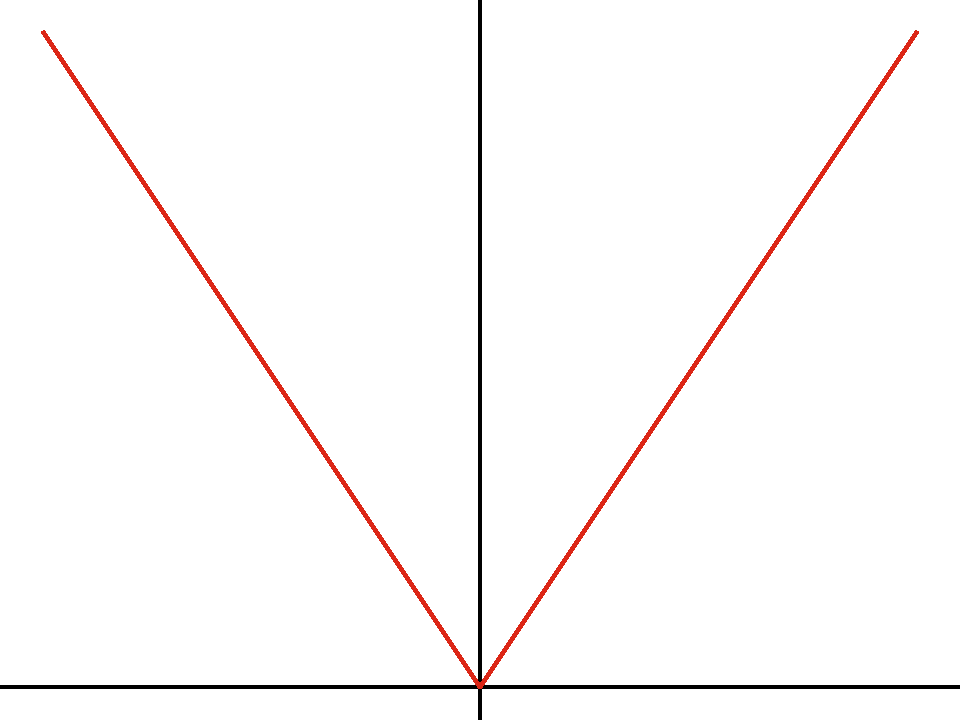
\includegraphics[scale=0.4]{gfx/ej1_2.pdf}
	\end{center}
	Se puede comprobar que la curva es de clase $\claseck{2}$, pero la gráfica es la misma que la de la función valor absoluto, que no es diferenciable en $x=0$. En este ``pico'' la derivada de la curva es $(0, 0)$.
\end{ejem}
La situación de este ejemplo es algo que intuitivamente queremos evitar: contradice la noción de ser \textit{suave}. La causa de este problema es que en este punto no existe una recta tangente bien definida, ya que el vector derivada es nulo. Solo nos interesa trabajar con curvas en las que esto no pase:

\begin{define}
	Una curva diferenciable $\alpha: I \rightarrow \reales^{n}$ se dice \textbf{regular} si $\alpha(t) \neq 0$ para todo $t \in I$. 
\end{define}

Una curva regular es tal que todo punto de la traza tiene por lo menos una recta tangente. Esto no significa que necesariamente sea única, como se puede apreciar en el ejemplo de la lemniscata de Bernoulli (en el punto de autointersección).\\ 

Ahora nuestro objetivo es establecer un parámetro que nos proporcione una forma ``natural'' de trabajar con una curva. De esta manera a una traza resultante de alguna curva regular le asignaremos una curva de alguna manera canónica (aunque esto no sea del todo posible, se ve más abajo).

\begin{define}
	Dada una curva diferenciable $\alpha: I \rightarrow \reales^{n}$ definimos su \textbf{longitud} desde $a$ hasta $b$ con $a\leq b \in I$ como la cantidad $\int_a^b |\alpha' (t)| dt$, y la denotaremos como $L_{a}^{b} (\alpha)$. 
\end{define}

Aquí damos una definición de longitud. Se podría demostrar que el producto escalar sobre $\reales^{n}$ da lugar (usando la definición de integral de Riemann) a está fórmula, pero nosotros no demostraremos esto.\\ 
Esta noción proporciona una invariante de una curva:

\begin{prop}
	Sea $\alpha: I \rightarrow \reales^{n}$ una curva diferenciable y $\beta: J \rightarrow \reales^{n}$ una reparametrización de $\alpha$. Si $t_0, t_1 \in I$, $s_0, s_1 \in J$ son tales que $\alpha(t_0) = \beta(s_0)$ y $\alpha(t_1) = \beta(s_1)$ entonces $L_{t_0}^{t_1} (\alpha) = L_{s_0}^{s_1} (\beta)$.
\end{prop}

\begin{define}
	Una curva diferenciable $\alpha: I \rightarrow \reales^{n}$ se dice \textbf{parametrizada por la longitud del arco} o \textbf{natural} si se tiene $|\alpha' (t)| = 1$ en todo $I$.
\end{define}

Esto nos dará para cada traza una curva ideal:

\begin{prop}\label{prop_arco_param}
	Para toda curva diferenciable regular existe una reparametrización por la longitud del arco.
\end{prop}

\begin{proof}
	La demostración nos enseña también como computar esta reparametrización. Sean $\alpha : I \rightarrow \reales$ una curva regular y $L : I \rightarrow J$ definida como $L(t) = L_{t_0}^{t}(\alpha)$ para algún $t_0 \in I$ fijo. $L$ es una función diferenciable y estrictamente creciente ya que la curva $\alpha$ es regular, por tanto tendrá una inversa que llamamos $s(t) = L^{-1} (t)$. Mediante la regla de la cadena es rutinario comprobar que $\beta : J \rightarrow \reales$ definida por $\beta(t) = \alpha(s(t))$ es una reparametrización de $\alpha$ y que $|\beta'(t)| = 1$ para todo $t \in J$.
\end{proof}

\begin{define}
	La aplicación $s$ de la demostración anterior se denomina \textbf{parámetro longitud de arco}.
\end{define}

La última proposición demuestra que siempre es posible encontrar una reparametrización de una curva regular de manera que el vector derivada sea siempre unitario. Es posible encontrar más de una para cada curva:

\begin{ejem}
	La circunferencia $\alpha(t) = (\cos t, \sin t)$ definida en todo $\reales$ está parametrizada por la longitud del arco (como se puede comprobar). La curva $\beta(t) = (\cos (-t), \sin (-t))$ definida en $\reales$ también es natural y es una reparametrización de $\alpha$ mediante $f(t) = -t$. 
\end{ejem}

Así, hablaremos de \textit{una} parametrización por arco.\\ 

Finalmente en esta sección hablamos de curvas cerradas. Intuitivamente, una curva cerrada es una curva $\alpha$ definida sobre un intervalo cerrado $[a, b]$ con $a,b \in \reales$ y $a < b$ tal que $\alpha(a) = \alpha(b)$. Esta definición no es perfecta:

\begin{ejem}
	
\end{ejem}

En vista de esto, es necesario añadir algo más a la definición:

\begin{define}
	Una curva diferenciable $\alpha: I \rightarrow \reales^{n}$ con $I = [a, b]$ intervalo cerrado con $a < b$ ambos reales se dice \textbf{cerrada} si se cumple $\alpha^{(m)}(a) = \alpha^{(m)}(b)$ para todo $m \in \naturales$.
\end{define}

Solo demostraremos la siguiente proposición:

\begin{prop}
	Sea $\alpha: [a, b] \rightarrow \reales^{n}$ una curva diferenciable cerrada. Entonces existe otra curva diferenciable $\beta: \reales \rightarrow \reales^{n}$ tal que:
	\begin{enumerate}
		\item
		$\beta^{(m)}(t) = \alpha^{(m)}(t)$ para todo $t \in [a, b]$ y $m \in \naturales$.
		\item
		$\beta$ es una aplicación periódica de periodo $b-a$.
	\end{enumerate}
\end{prop}













\section{Curvatura de curvas planas}
El objetivo final de esta sección será establecer una caracterización de las curvas en $\reales^{2}$, y crear un sistema de coordenadas ``local'' para describir curvas. En esta sección asumiremos que las curvas con las que tratamos son por lo menos de clase $\claseck{2}$, e inicialmente que están parametrizadas por la longitud del arco.\\ 

Para lograr nuestro objetivo, estudiaremos el comportamiento del vector derivada. Para esto introducimos una definición:

\begin{define}\label{def_curva_vector_tangente1}
	Si $\alpha: I \rightarrow \reales^2$ es una curva natural y $s_0 \in I$ entonces definimos el \textbf{vector tangente unitario} en $s_0$ como $T(s_0) = \alpha'(s_0)$.
\end{define}

Como $\alpha$ es natural, el módulo del vector derivada siempre es $1$ y por tanto no nos tenemos que preocupar de normalizar el vector. Antes de seguir necesitamos unos resultados pequeños:

\begin{lemma}\label{lemma_vectores_unitarios}
	Si $\alpha: I \rightarrow \reales^{n}$ es cualquier función vectorial tal que $|\alpha(t)| = 1$ para todo $t \in I$ entonces $\langle \alpha(t),\alpha'(t) \rangle = 0$ para todo $t \in I$. Es decir, el vector derivada y el vector son ortogonales en todo el dominio.
\end{lemma}

\begin{lemma}\label{lemma_direccion_normal}
	Existen exactamente dos aplicaciones $J:\reales^{2} \rightarrow \reales^{2}$ que satisfacen:
	\begin{enumerate}
		\item
		$|J(x, y)| = |(x, y)|$ para todo $(x, y) \in \reales^{2}$.
		\item
		$J(x, y)$ es ortogonal a $(x, y)$ para todo $(x, y) \in \reales^{2}$.
		\item
		$J$ es continua en todo $\reales^{2}$.
	\end{enumerate}
\end{lemma}

El primer lema es algo que constantemente usaremos. El segundo lema no es tan útil y solo nos sirve para darle algo más de sentido a esta definición:

\begin{define}
	La aplicación $J:\reales^{2} \rightarrow \reales^{2}$ dada por la expresión $J(x, y) = (-y, x)$ la denominaremos \textbf{orientación normal elegida}.
\end{define}

La orientación normal elegida es una de las dos aplicaciones de la proposición \eqref{lemma_direccion_normal}. El lema existe para saber que existen dos formas ``canónicas'' de elegir una orientación para los vectores normales en $\reales^2$, y la definición nos sirve para definir el vector normal:

\begin{define}\label{def_curva_vector_normal1}
	Si $\alpha: I \rightarrow \reales^2$ es una curva natural y $s_0 \in I$ entonces definimos el \textbf{vector normal unitario} en $s_0$ como $n(s_0) = J(T(s_0))$.
\end{define}

Como $T(s_0)$ es unitario, $n(s_0)$ también lo es. Al ser estos dos vectores ortogonales, podemos definir una base vectorial de $\reales^2$:

\begin{define}
	Dada una curva natural $\alpha: I \rightarrow \reales^2$, se define la \textbf{base de Frenet} (o diedro) en cada punto $s_0 \in I$ a la base vectorial $\{T(s_0), n(s_0) \}$.
\end{define}

La base de Frenet es ortonormal, y nos va a permitir definir el concepto más importante de esta sección:

\begin{define}\label{def_curva_curvatura1}
	Se define la \textbf{curvatura} de $\alpha$ en $s_0 \in I$ como el número $\kappa(s_0)$ tal que $T'(s_0) = \kappa(s_0)n(s_0)$.
\end{define}

\begin{proof}
	Vamos a demostrar la existencia de tal número. Fijamos $s_0 \in I$, y por el lema \eqref{lemma_vectores_unitarios} $\langle T'(s_0), T(s_0) \rangle = 0$. Considerando la base de Frenet, sabemos las coordenadas de un vector cualquiera en una base ortonormal: 
	\begin{equation*}
		T'(s_0) = \langle T'(s_0), T(s_0) \rangle T(s_0) + \langle T'(s_0), n(s_0) \rangle n(s_0)
	\end{equation*}		
	y así $T'(s_0) = \langle T'(s_0), n(s_0) \rangle n(s_0)$. $\kappa(s_0) = \langle T'(s_0), n(s_0) \rangle$ es lo que buscamos.
\end{proof}

La curvatura mide cuanto de \textit{curvada} esta una curva. Son también importantes las siguientes fórmulas:

\begin{prop}[Fórmulas de Frenet]
	Para toda curva natural:
	\begin{eqnarray}
		T' = \kappa n \label{eq_frenet2d_1}\\ 
		n' = -\kappa T \label{eq_frenet2d_2}
	\end{eqnarray}
\end{prop}

\begin{proof}
	La ecuación \eqref{eq_frenet2d_1} es la definición de curvatura. Para \eqref{eq_frenet2d_2}, como $\{T(s), n(s) \}$ es una base para todo $s \in I$ podemos escribir
	\begin{equation*}
		n'(s) = \langle n'(s), T(s) \rangle T(s) + \langle n'(s), n(s) \rangle n(s)
	\end{equation*}
	Por ser $n(s)$ unitario, aplicando el lema \eqref{lemma_vectores_unitarios} obtenemos $\langle n'(s), n(s) \rangle = 0$. Sabemos que $\langle T(s), n(s) \rangle = 0$. Derivando esta expresión y simplificando obtenemos:
	\begin{equation*}
	\begin{split}
		0 & = \langle T'(s), n(s) \rangle + \langle T(s), n'(s) \rangle \\ 
		& = \langle \kappa(s)n(s), n(s) \rangle + \langle T(s), n'(s) \rangle \\
		& = \kappa(s) + \langle T(s), n'(s) \rangle
		\Rightarrow \langle T(s), n'(s) \rangle = -\kappa(s)
	\end{split}
	\end{equation*}
	y así:
	\begin{equation*}
		n'(s) = -\kappa(s) T(s)
	\end{equation*}
\end{proof}

\begin{ejem}
	Vamos a demostrar que $\kappa \equiv 0$ si y solo sí $\alpha$ es un segmento (posiblemente no acotado) de recta. Sea $\alpha : (a, b) \rightarrow \reales^2$ una curva natural con curvatura $0$. Por la definición de curvatura $\alpha'' = T' = \kappa n = 0$. Integrando ambas componentes de $\alpha$ podemos escribir $\alpha(t) = ct + d$ para todo $t \in (a, b)$ y algunas constantes $c, d \in \reales^2$, y por tanto $\alpha$ es o un punto (en cuyo caso $\alpha'(t) = 0$ y por tanto $\alpha$ no sería regular) o un segmento de recta. Conversamente, si $\alpha$ es un segmento de recta parametrizado por la longitud del arco existirá una reparametrización en la que tengamos $\alpha(t) = ct + d$ para todo $t \in (a, b)$ con $c, d \in \reales^2$ constantes con $|c| = 1$. Por la definición de la curvatura $\kappa(t) = |T'(t)| = |\alpha''(t)| = 0$.
\end{ejem}

Es fácil extender los conceptos definidos para curvas naturales a curvas regulares que no están parametrizadas por la longitud del arco.

\begin{define}
	Sea $\alpha : I \rightarrow \reales^2$ una curva regular. Por \eqref{prop_arco_param} existe una reparametrización natural $\beta : J \rightarrow \reales^2$ bajo un parámetro $L : I \rightarrow J$. Definimos:
	\begin{enumerate}
		\item
		El \textbf{vector tangente unitario} de $\alpha$ en $t_0$ como $T_{\alpha}(t_0) = T_{\beta}(L(t_0))$ donde $T_{\beta}(L(t_0))$ es el vector tangente unitario a $\beta$ en $L(t_0)$ definido en \eqref{def_curva_vector_tangente1}.
		\item
		El \textbf{vector normal unitario} de $\alpha$ en $t_0$ como $n_{\alpha}(t_0) = n_{\beta}(L(t_0))$ donde $n_{\beta}(L(t_0))$ es el vector normal unitario a $\beta$ en $L(t_0)$ definido en \eqref{def_curva_vector_normal1}.
		\item
		La \textbf{curvatura} de $\alpha$ en $t_0$ como $\kappa_{\alpha}(t_0) = \kappa_{\beta}(L(t_0))$ donde $\kappa_{\beta}(L(t_0))$ es la curvatura a $\beta$ en $L(t_0)$ definido en \eqref{def_curva_curvatura1}.
	\end{enumerate}
\end{define}

Es habitual poner en el subíndice de $T$, $n$ y $\kappa$ a que curva nos referimos para hacer la lectura más fácil.\\ 
En términos de cálculo, calcular la parametrización por longitud de arco de una curva es algo que puede resultar complicado. La integral de la longitud puede resultar ser no elemental, y después es probable que la inversa de la función longitud tampoco sea elemental. Es entonces sorprendente que para la curvatura exista una fórmula cerrada para calcularla en cualquier parametrización.

\begin{prop}
	Sea $\alpha : I \rightarrow \reales^2$ una curva regular no necesariamente natural. Entonces:
	\begin{equation*}
	\begin{split}
		& T_{\alpha}(t_0) = \frac{\alpha'(t_0)}{|\alpha'(t_0)|} \\ 
		& n_{\alpha}(t_0) = \frac{J(\alpha'(t_0))}{|\alpha'(t_0)|} \\ 
		& \kappa_{\alpha(t_0)} = \frac{1}{|\alpha'(t_0)|^3} \langle J(\alpha'(t_0)), \alpha''(t_0) \rangle
	\end{split}
	\end{equation*}
	para todo $t_0 \in I$. 
\end{prop}

Para terminar esta sección, constatamos que la longitud de arco y la curvatura definen completamente una curva:

\begin{theorem}
	Sea $\kappa : I \rightarrow \reales$ una función continua. Entonces existe una curva $\alpha : I \rightarrow \reales^2$ parametrizada por la longitud del arco tal que $\kappa_{\alpha}(t) = \kappa(t)$ para todo $t \in I$. Además, si $\beta : I \rightarrow \reales^2$ es otra curva natural con la misma curvatura que $\alpha$, existe un movimiento rígido $M$ del plano tal que $\beta = M \circ \alpha$.
\end{theorem}	
	
\begin{theorem}
	Sea $\kappa : I \rightarrow \reales$ y $s : I \rightarrow \reales$ dos funciones continuas. Entonces existe una curva $\alpha : I \rightarrow \reales^2$ tal que $\kappa_{\alpha}(t) = \kappa(t)$ y $L_{t_0}^{t} = s(t)$ para todo $t \in I$, y un $t_0 \in I$ fijo.
\end{theorem}

La longitud del arco y la curvatura entonces dan un sistema de coordenadas local para la curva.









\section{Curvatura y torsión de curvas alabeadas}
Las curvas alabeadas son las curvas $\alpha : I \rightarrow \reales^3$. \\ 
Para curvas planas, hemos estudiado la variación de la base de Frenet para estudiar la curva. En ese caso la base tenía $2$ vectores, y sus derivadas vienen tienen las relaciones dadas en \eqref{eq_frenet2d_1} y \eqref{eq_frenet2d_2}. En $\reales^3$ una base vectorial necesita tener $3$ vectores. Si tomamos el vector tangente a una curva (es decir, el vector derivada) el conjunto de los vectores ortogonales a él es un espacio vectorial de dimensión $2$, y por tanto no podemos ``elegir'' un solo vector como hacíamos con el automorfismo $J$ de la sección anterior. Esto cambiara las cosas ligeramente, entre otras hará que la curvatura no tenga signo y sea una cantidad no negativa. \\
Como al principio de la anterior sección, primero trabajamos con curvas parametrizadas por la longitud de arco.

\begin{define}
	Una curva $\alpha : I \rightarrow \reales^3$ regular se dice \textbf{1-regular} si y solo si $\alpha''(s)\neq 0\ \forall s \in I$ .
\end{define}

Para poder definir una base de Frenet en curvas alabeadas necesitamos trabajar con curvas 1-regulares. Asumiremos por ahora que las curvas con las que trabajamos son 1-regulares.

\begin{define}
	Dada una curva $\alpha : I \rightarrow \reales^3$ 1-regular natural definimos:
	\begin{itemize}
		\item
		El \textbf{vector tangente unitario} en $s_0 \in I$ como $T(s_0) = \alpha'(s_0)$.
		\item
		La \textbf{curvatura} en $s_0 \in I$ como el número $\kappa(s_0) = |\alpha''(s_0)| = |T'(s_0)|$.
		\item
		El \textbf{vector normal unitario} en $s_0 \in I$ como el vector $n(s_0)$ tal que $T'(s_0) = \kappa(s_0)n(s_0)$.
		\item
		El \textbf{vector binormal unitario} en $s_0 \in I$ como $b(s_0) = T(s_0) \wedge n(s_0)$.
		\item
		La tupla $\{T(s_0), n(s_0), b(s_0)\}$ es una base ortonormal de $\reales^3$ para todo $s_0 \in I$ y la denominamos \textbf{base} o \textbf{triedro de Frenet}.
	\end{itemize}
\end{define}

Si $\alpha$ no fuera 1-regular, el vector binormal unitario sería el vector nulo, y por tanto ni sería unitario ni podríamos formar la base de Frenet.

\begin{prop}
	Existe un número $\tau(s_0)$ para cada $s_0 \in I$ tal que $b'(s_0) = \tau(s_0)n(s_0)$. A este número se le llama la \textbf{torsión}.
\end{prop}

\begin{proof}
	Derivando la definición de $b(s)$ obtenemos:
	\begin{equation*}
		b'(s_0) = T'(s_0) \wedge n(s_0) + T(s_0) \wedge n'(s_0) = T(s_0) \wedge n'(s_0)
	\end{equation*}
	donde $T'(s_0) \wedge n(s_0) = 0$ por la definición del vector normal. Por el lema \eqref{lemma_vectores_unitarios} $n'(s_0)$ es ortogonal a $n(s_0)$ y por ser $\{T(s_0), n(s_0), b(s_0)\}$ base ortonormal, $n'(s_0)$ es paralelo al subespacio generado por $T(s_0)$ y $b(s_0)$. Así, si $n'(s_0)$ no es paralelo a $T(s_0)$, $T(s_0) \wedge n'(s_0)$ será perpendicular a este subespacio y por tanto múltiplo de $n(s_0)$. Si $n(s_0)$ fuera paralelo a $T(s_0)$, $T(s_0) \wedge n'(s_0)$ sería cero.
\end{proof}

La curvatura y la torsión son las dos funciones que necesitamos para caracterizar una curva alabeada (junto con la longitud de arco). Primero vemos el resultado análogo a las fórmulas de Frenet:

\begin{theorem}
	Si $\alpha: I \rightarrow \reales^3$ es una curva natural 1-regular se cumple:
	\begin{equation*}
		\begin{bmatrix}
			T' \\
			n' \\
			b' 
		\end{bmatrix}
		=
		\begin{bmatrix}
			0 & \kappa & 0 \\
			-\kappa & 0 & -\tau \\
			0 & \tau & 0 
		\end{bmatrix}
		\begin{bmatrix}
			T \\
			n \\
			b 
		\end{bmatrix}
	\end{equation*}
\end{theorem}

\begin{proof}
	Las fórmulas correspondientes a la primera y última fila de la matriz son la definición de la curvatura y la torsión. Solo hace falta demostrar la segunda. Por la base de Frenet tenemos $\langle T(s_0), n(s_0) \rangle = 0$ y $\langle b(s_0), n(s_0) \rangle = 0$. Derivando y reordenando obtenemos $\langle T(s_0), n'(s_0) \rangle = - \langle T'(s_0), n(s_0) \rangle = -\kappa(s_0)$ y $\langle b(s_0), n'(s_0) \rangle = - \langle b'(s_0), n(s_0) \rangle = -\tau(s_0)$. Por ser la base de Frenet ortonormal y $n'(s_0)$ ortogonal a $n(s_0)$ tenemos $n'(s_0) = \langle T(s_0), n'(s_0) \rangle T(s_0) + \langle b(s_0), n'(s_0) \rangle b(s_0) = -\kappa(s_0)T(s_0) - \tau(s_0) b(s_0)$.
\end{proof}

Todo esto se extiende de forma similar a curvas que no están parametrizadas por la longitud del arco, y de la misma forma tenemos las siguientes fórmulas:

\begin{prop}
	Sea $\alpha : I \rightarrow \reales^3$ una curva regular y 1-regular no necesariamente natural. Se cumple:
	\begin{equation*}
	\begin{split}
		& T_{\alpha} = \frac{\alpha'}{|\alpha'|} \\ 
		& b_{\alpha} = \frac{\alpha' \wedge \alpha''}{|\alpha' \wedge \alpha''|}\\ 
		& n_{\alpha} = b_{\alpha} \wedge T_{\alpha}\\
		& \kappa_{\alpha} = \frac{1}{|\alpha'|^3} |\alpha' \wedge \alpha''|\\
		& \tau_{\alpha} = -\frac{[\alpha', \alpha'', \alpha''']}{|\alpha' \wedge \alpha''|^2}
	\end{split}
	\end{equation*}
\end{prop}








\section{La definición de superficie regular}
El concepto de superficie regular es una ``versión bidimensional'' del concepto de curva regular. Intuitivamente una curva es un objeto unidimensional continuo y suave, mientras que una superficie será un objeto bidimensional con características similares. Resulta que, no tan sorprendemente, tratar con este tipo de geometría correctamente es más complicado que trabajar con la geometría de las curvas. Además, la definición de superficie será una definición ``geométrica'', contrariamente al punto de vista dinámico que hemos usado para curvas: para nosotros, una curva era una aplicación diferenciable, más que un subconjunto de $\reales^n$. Esto equivale a hablar de la traza de la curva con un sistema de coordenadas predeterminado dado por la aplicación en sí. Contrasta por ejemplo a como se tratan los sistemas de coordenadas (bases) en espacios vectoriales: tenemos un objeto del que podemos hablar sin asignarle coordenadas y además dependiendo de que queramos hacer con él le podemos aplicar las coordenadas que más nos convengan. En el caso de las curvas esto no es muy atractivo, pero con superficies puede resultar más interesante.

\begin{define}
	Llamamos a un subconjunto no vacío $S \subseteq \reales^3$ una \textbf{superficie regular} si para todo $p \in S$ existe un abierto no vacío $U \in \reales^2$ y un homeomorfismo topológico $X: U \rightarrow X(U) \subseteq S$ tal que:
	\begin{itemize}
		\item
		$X(U)$ es un entorno abierto de $p$ en la topología heredada de $S$ en $\reales^3$.
		\item
		$X$ como aplicación $X: U \rightarrow \reales^{3}$ es diferenciable y la diferencial $dX_q$ es inyectiva para todo $q \in X(U)$.
	\end{itemize}
\end{define}

\begin{prop}
	Sea $S$ una superficie regular y $X: U \rightarrow S$, $Y: V \rightarrow S$ dos parametrizaciones regulares alrededor de $p \in S$. Entonces la aplicación $X^{-1} \circ Y : V \rightarrow U$ es una aplicación diferenciable.
\end{prop}

\section{Plano tangente y aplicaciones diferenciables}
\begin{define}
	Sea $S$ una superficie regular y $p \in S$. Decimos que $v \in \reales^3$ es un \textbf{vector tangente} si existe una parametrización regular $X: U \rightarrow S$ alrededor de $p$ y una curva regular $\alpha: (-\varepsilon, \varepsilon) \rightarrow U$ tal que $(X \circ \alpha)' (0) = v$.
\end{define}
\section{Primera forma fundamental}
\section{Segunda forma fundamental}
\section{Indicatriz de Dupin}

\section{Espacios seudoeuclídeos}
\section{Hipersuperficies}



















\end{document}